\documentclass[aspectratio=169,11pt]{beamer}

% Overleaf: compiler pdfLaTeX. All image paths are relative to main.tex.
\usepackage{iftex}
\ifPDFTeX
  \usepackage[T1]{fontenc}
  \usepackage[utf8]{inputenc}
  \usepackage{lmodern}
\else
  \usepackage{fontspec}
  \setsansfont{lmsans10-regular.otf}[
    BoldFont=lmsans10-bold.otf,
    ItalicFont=lmsans10-oblique.otf,
    BoldItalicFont=lmsans10-boldoblique.otf]
  \setmainfont{lmroman10-regular.otf}[
    BoldFont=lmroman10-bold.otf,
    ItalicFont=lmroman10-italic.otf,
    BoldItalicFont=lmroman10-bolditalic.otf]
  \setmonofont{lmmono10-regular.otf}
\fi
\usepackage[polish]{babel}
\usepackage{graphicx}
\usepackage{booktabs}
\usepackage{array}
\usepackage{ragged2e}

\definecolor{Forest}{HTML}{245647}
\definecolor{Ink}{HTML}{202B28}
\definecolor{Muted}{HTML}{66716B}
\definecolor{Accent}{HTML}{A54832}
\definecolor{Paper}{HTML}{F7F8F4}
\setbeamercolor{normal text}{fg=Ink,bg=white}
\setbeamercolor{structure}{fg=Forest}
\setbeamercolor{frametitle}{fg=Forest,bg=white}
\setbeamercolor{title}{fg=Forest}
\setbeamercolor{alerted text}{fg=Accent}
\setbeamercolor{block title}{fg=Forest,bg=Paper}
\setbeamercolor{block body}{fg=Ink,bg=Paper}
\setbeamerfont{normal text}{size=\normalsize}
\setbeamerfont{title}{size=\fontsize{28}{32}\selectfont,series=\bfseries}
\setbeamerfont{frametitle}{size=\fontsize{21}{25}\selectfont,series=\bfseries}
\setbeamerfont{block title}{series=\bfseries}
\setbeamertemplate{navigation symbols}{}
\setbeamertemplate{itemize item}{\color{Forest}\small\textbullet}
\setbeamertemplate{itemize subitem}{\color{Forest}\small\textbullet}
\setbeamertemplate{frametitle}{\vspace{0.25cm}\insertframetitle\par\vspace{0.12cm}}
\setbeamersize{text margin left=0.65cm,text margin right=0.65cm}
\setbeamertemplate{footline}{%
  \hfill\textcolor{Muted}{\scriptsize\insertframenumber/\inserttotalframenumber}%
  \hspace{0.65cm}\vspace{0.25cm}}
\setlength{\parskip}{0.15cm}
\graphicspath{{images/}}
\hypersetup{colorlinks=true,urlcolor=Forest,linkcolor=Forest}
\newcommand{\src}[1]{\par\vspace{0.12cm}{\fontsize{7}{9}\selectfont\color{Muted}#1\par}}
\newcommand{\shot}[3]{%
  \centering\includegraphics[width=\linewidth,height=4.55cm,keepaspectratio]{#1}\par
  \vspace{0.12cm}{\small\bfseries #2}\par{\scriptsize\color{Muted}#3}\par}
\newcommand{\modelgemma}{Gemma 3 4B}
\newcommand{\modelqwen}{Qwen3-VL 4B Instruct}

\title{Import przepisu\\ze screena}
\subtitle{MealBrAIn: pierwsza próba scenariusza S1}
\author{}
\date{}

\begin{document}

% 1
\begin{frame}[plain]
  \vspace{0.55cm}
  {\large\color{Muted}MealBrAIn\par}
  \vspace{0.35cm}
  {\usebeamerfont{title}\color{Forest}Import przepisu\\ze screena\par}
  \vspace{0.3cm}
  {\large Pierwsza próba S1 z lokalnymi modelami Ollamy\par}
  \vfill
  {\small\color{Muted}Cel: odczytać widoczne dane i zachować braki przepisu.\par}
  \note{Przedstawiam część S1, czyli import z obrazu. Wynik powinien pasować do wspólnego RecipeDraft używanego w imporcie tekstowym S3. To pierwsza próba jednej konfiguracji, a nie ukończony moduł. Źródła: sources/raport.md i sources/protokol.md.}
\end{frame}

% 2
\begin{frame}{Przebieg testu}
  \begin{columns}[T,onlytextwidth]
    \begin{column}{0.53\textwidth}
      \textbf{6 obrazów, 2 modele, 12 odczytów}
      \begin{enumerate}
        \setlength{\itemsep}{0.16cm}
        \item Odczyt screenów i zapis oczekiwanych danych przed próbą.
        \item Zamrożenie obrazów, wzorców, promptu i ustawień.
        \item Osobne żądanie dla każdego obrazu, bez historii innych przepisów.
        \item Walidacja w C\# i ocena zgodności odpowiedzi z obrazem.
      \end{enumerate}
    \end{column}
    \begin{column}{0.43\textwidth}
      \textbf{Modele w Ollamie}
      \par\modelgemma
      \par\modelqwen
      \vspace{0.18cm}

      {\small
      \begin{tabular}{@{}ll@{}}
        Temperatura & 0 \\
        Kontekst & 16\,384 tokeny \\
        Limit odpowiedzi & 4\,096 tokenów \\
        Oczekiwany wynik & \texttt{RecipeDraft v1}
      \end{tabular}\par}
      \vspace{0.15cm}
      {\small Jeden przebieg na model. Bez rozgrzewki i automatycznych ponowień.}
    \end{column}
  \end{columns}
  \note{Modele otrzymywały wyłącznie obraz, wspólny prompt S1 oraz schemat odpowiedzi. Nie dostawały wzorców ani transkrypcji przygotowanych do oceny. Gemma działała pierwsza, potem Qwen. Ustawienia: think pominięte, keep alive 10 minut, JSON Schema w parametrze format. Ollama 0.40.11, .NET 10.0.13. Źródło: sources/protokol.md oraz sources/raport.md.}
\end{frame}

% 3
\begin{frame}{Prompt S1: fragmenty użytej instrukcji}
  {\small Ten sam prompt systemowy i schemat \texttt{RecipeDraft v1} dla obu modeli.\par}
  \begin{quote}
    \small
    „Zwróć wyłącznie zwarty JSON zgodny z podanym schematem RecipeDraft v1.”

    „Źródłem danych jest tylko widoczna treść obrazu.”

    „Wszystkie wymagane pola muszą być obecne; niewiadome zapisuj jako \texttt{null}.”

    „Nie uzupełniaj \texttt{unknown} domyślną porcją.”

    „Nigdy nie zatwierdzasz i nie zapisujesz przepisu.”
  \end{quote}
  \vspace{0.05cm}
  \textbf{Wiadomość użytkownika i załączony obraz}
  \par{\small „Odczytaj przepis z załączonego obrazu zgodnie ze schematem. Nie uzupełniaj niewidocznych danych.”}
  \note{To dosłowne fragmenty promptu S1 v1 użytego w badaniu, a nie instrukcja poprawiona po wynikach. Pełny tekst jest w sources/image-extraction-prompt-v1.txt. Kod dołączał do wiadomości systemowej także schemat, dostępny w sources/recipe-draft-v1.schema.json. Wiadomość użytkownika była stała, a obraz znajdował się w polu images. Pełny prompt zawiera ponadto zasady odczytu ilości, czasów, cytatów, konfliktów i niekompletnych przepisów.}
\end{frame}

% 4
\begin{frame}{Materiał: niekompletne przepisy z Instagrama}
  {\small Pięć fragmentów przepisów i jeden kadr bez przepisu. Jeden obraz po angielsku, pięć z polskim tekstem lub interfejsem.\par}
  \vspace{0.15cm}
  \begin{columns}[T,onlytextwidth]
    \begin{column}{0.235\textwidth}
      \shot{makaron.jpg}{Makaron}{Przyprawy tylko w krokach}
    \end{column}
    \begin{column}{0.235\textwidth}
      \shot{bajgle.jpg}{Bajgle}{Ułamki i różne czasy}
    \end{column}
    \begin{column}{0.235\textwidth}
      \shot{kaszka.png}{Kaszka}{Lista bez instrukcji}
    \end{column}
    \begin{column}{0.235\textwidth}
      \shot{kluski.jpg}{Kluski leniwe}{Ilości w kilku miejscach}
    \end{column}
  \end{columns}
  \note{Galeria pokazuje układ źródeł, nie wymaga odczytywania wszystkich małych napisów podczas wystąpienia. Pełne obrazy są w katalogu images. Żaden z pięciu przepisów nie zawiera całego kompletu wymaganych danych. Brak jednostki lub kroków jest prawidłowym stanem wejścia. Nie badaliśmy jeszcze stron internetowych, rozmazanych cyfr, jawnych konfliktów ani ukrytych poleceń. Źródła obrazów: IMG_5281.JPEG, IMG_5283.JPEG, IMG_5284.PNG i IMG_5286.JPEG.}
\end{frame}

% 5
\begin{frame}{Batony: model dopisuje niewidoczne dane}
  \begin{columns}[T,onlytextwidth]
    \begin{column}{0.51\textwidth}
      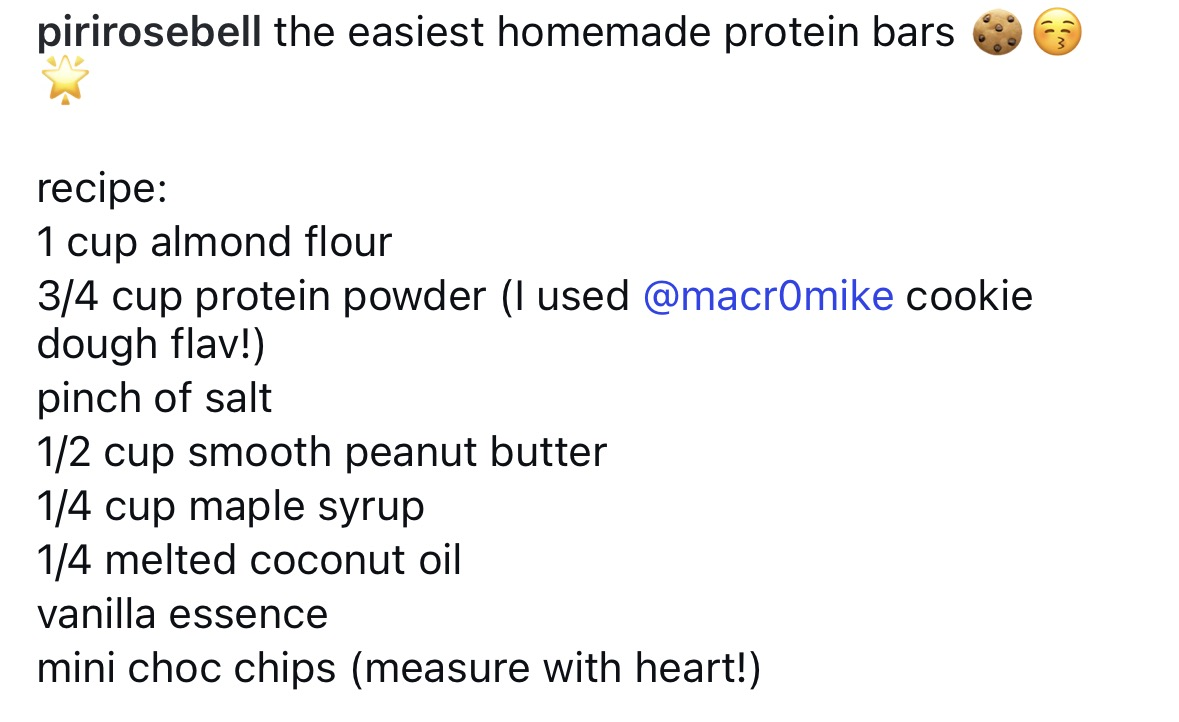
\includegraphics[width=\linewidth,height=4.7cm,keepaspectratio]{protein-bars.jpg}
      \src{S1-001 / IMG\_5280.JPEG}
    \end{column}
    \begin{column}{0.45\textwidth}
      \textbf{Co widać na screenie}
      \begin{itemize}
        \item \texttt{3/4 cup protein powder}
        \item \texttt{1/4 melted coconut oil}
        \item Brak kroków, porcji i czasu.
      \end{itemize}
      \vspace{0.1cm}
      \textbf{Co zwróciły modele}
      \begin{itemize}
        \item Gemma: \alert{0,375} zamiast 0,75 oraz instrukcja rozgrzania piekarnika.
        \item Oba modele dopisały olejowi jednostkę \alert{\texttt{cup}}.
      \end{itemize}
    \end{column}
  \end{columns}
  \vspace{0.15cm}
  \textbf{Oczekiwanie:} ilość oleju 0,25 z nieznaną jednostką, kroki puste.
  \note{Źródło jest niekompletne, ale nadaje się do importu z oznaczonymi brakami. Nie wolno dopisać cup tylko dlatego, że sąsiednie wiersze używają tej jednostki. Gemma wymyśliła cztery kroki, w tym piekarnik 350 stopni Fahrenheita lub 175 Celsjusza. Qwen poprawnie odczytał 0.75 i nie dopisał kroków, ale popełnił błąd jednostki oraz błędy formatu ilości. Źródła: sources/raport.md, sources/gemma-batony.json i sources/qwen-batony.json.}
\end{frame}

% 6
\begin{frame}{Sam kadr potrawy powinien dać \texttt{not\_recipe}}
  \begin{columns}[T,onlytextwidth]
    \begin{column}{0.29\textwidth}
      \centering
      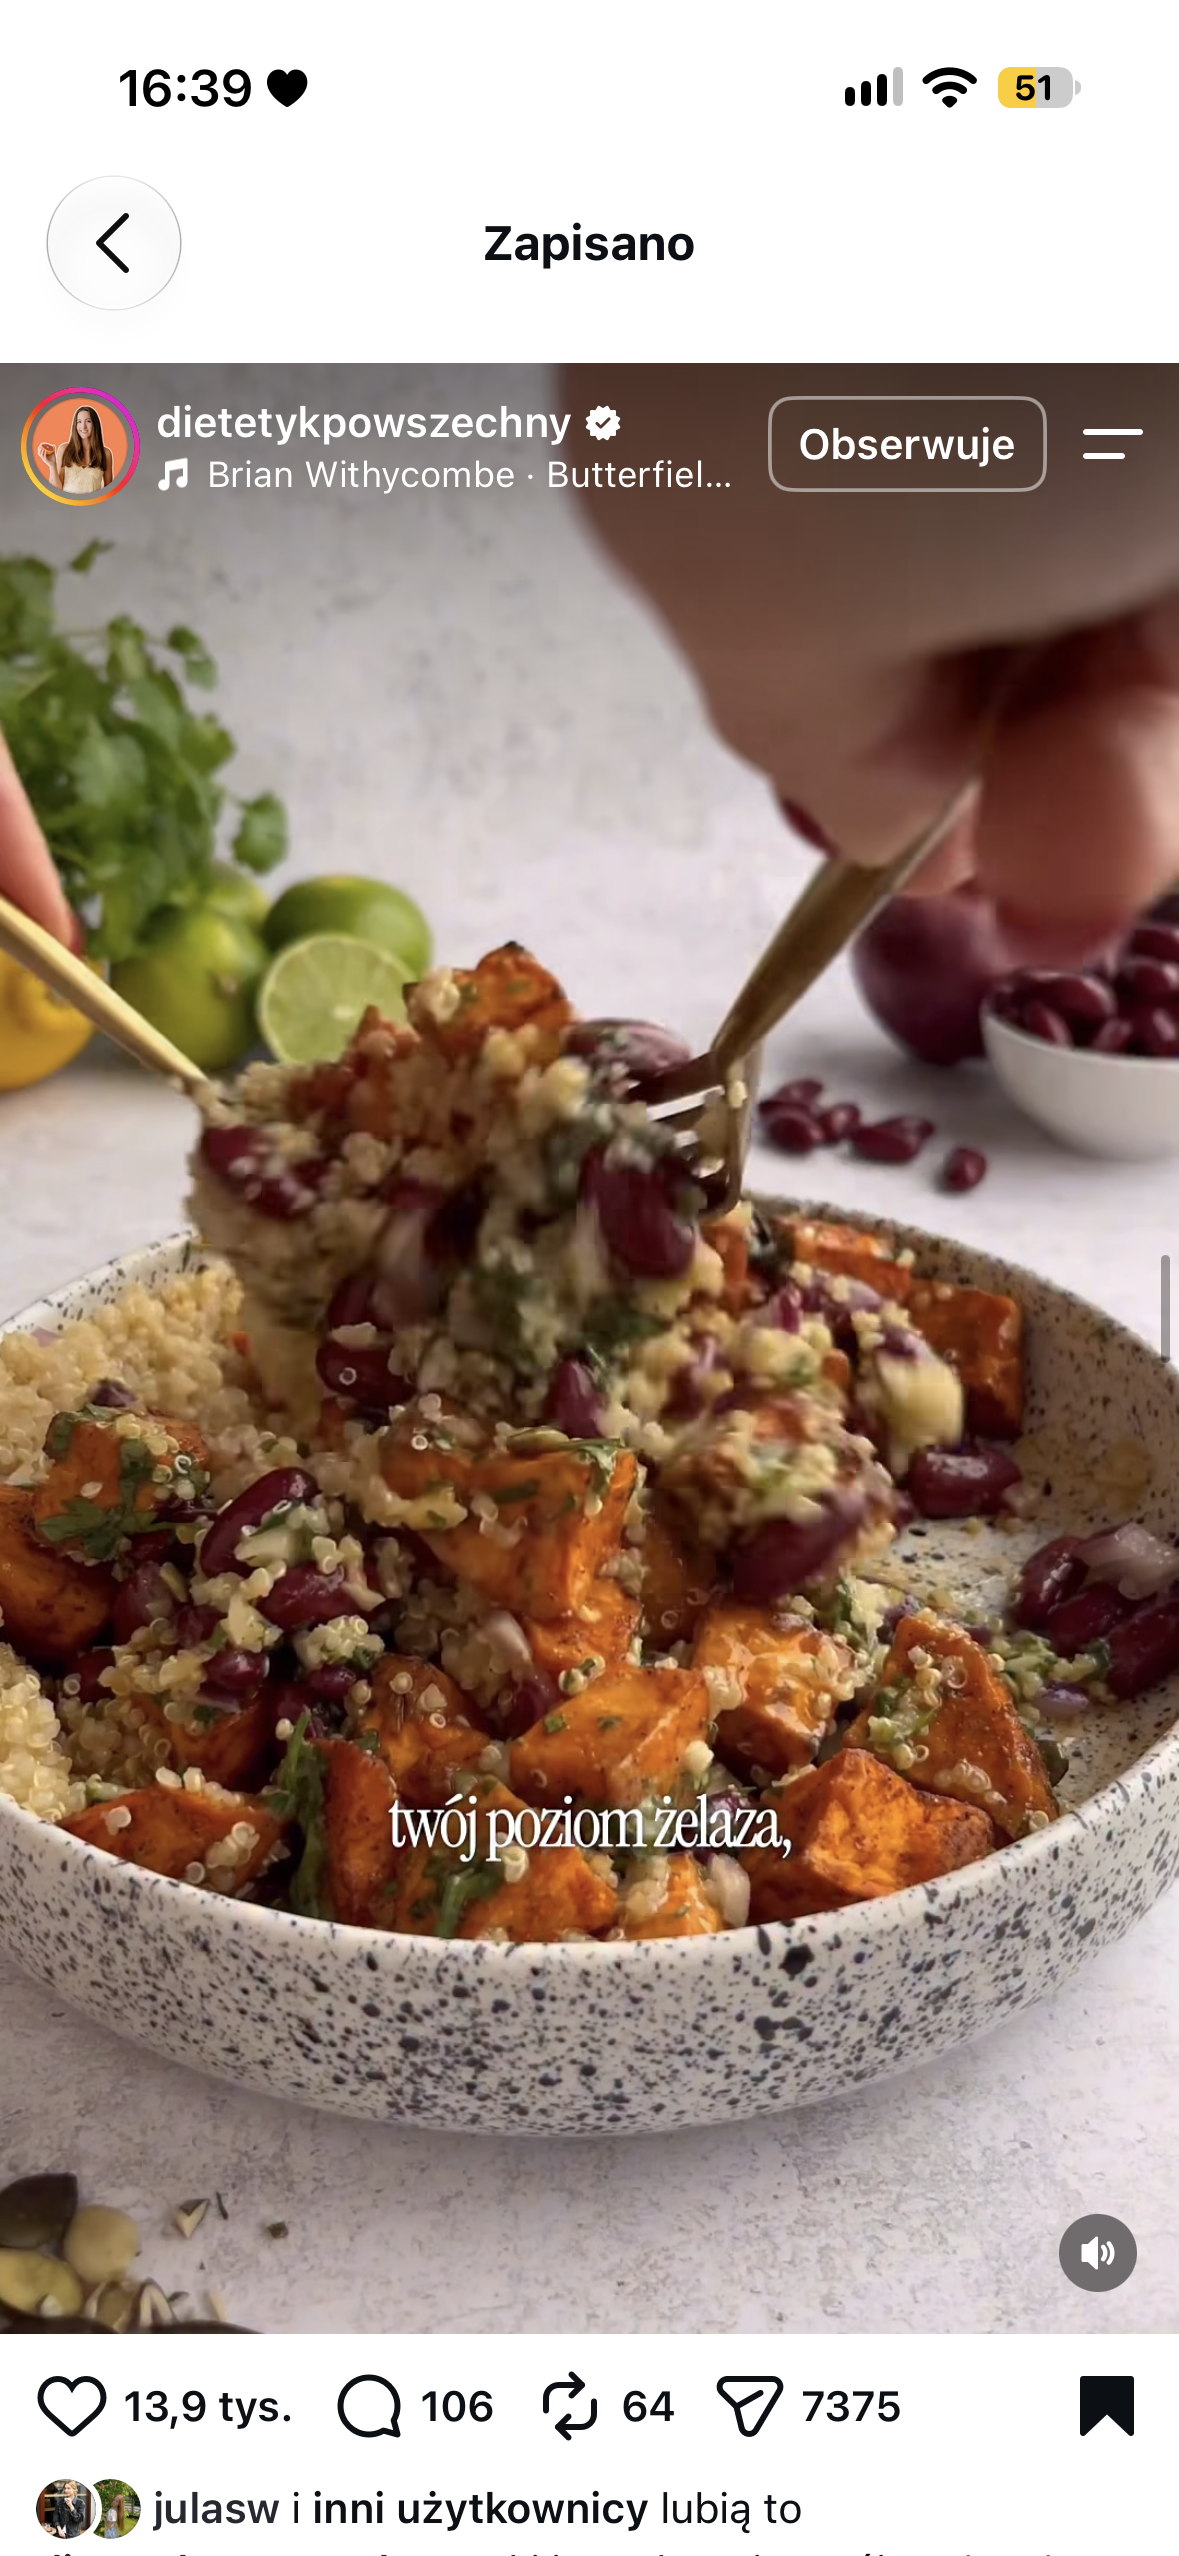
\includegraphics[width=\linewidth,height=5.65cm,keepaspectratio]{kadr-potrawy.png}
    \end{column}
    \begin{column}{0.66\textwidth}
      \textbf{Źródło}
      \par Zdjęcie potrawy i elementy Instagrama. Brak listy składników i instrukcji.

      \vspace{0.15cm}
      \textbf{\modelgemma}
      \par Dopisuje m.in. \alert{400 g fasoli}, szklankę ryżu i cztery kroki przygotowania.

      \vspace{0.15cm}
      \textbf{\modelqwen}
      \par Poprawnie zwraca \texttt{not\_recipe} oraz \texttt{recipe=null}.

      \vspace{0.12cm}
      {\small To jedyny w pełni zaliczony przypadek Qwena w tej próbie.}
    \end{column}
  \end{columns}
  \src{S1-005 / IMG\_5285.PNG. Oceniamy wyłącznie dostępny screen, nie cały post ani film.}
  \note{Nie próbujemy odgadywać przepisu na podstawie wyglądu jedzenia. Przypadek sprawdza zdolność powstrzymania się od zmyślenia danych. Gemma zwróciła dokument poprawny według reguł strukturalnych, mimo że jego treść nie miała źródła na obrazie. Qwen poprawnie odrzucił materiał. Źródła: sources/gemma-kadr.json, sources/qwen-kadr.json i sources/raport.md.}
\end{frame}

% 7
\begin{frame}{Poprawny JSON może łamać reguły przepisu}
  \textbf{Przykład Qwena: 1 cup almond flour}
  \vspace{0.15cm}

  \begin{center}
    \renewcommand{\arraystretch}{1.4}
    \begin{tabular}{@{}lcccc@{}}
      \toprule
      \texttt & \texttt{value} & \texttt{min} & \texttt{max} & \texttt{text} \\
      \midrule
      Wynik modelu & 1 & \alert{1} & \alert{1} & \alert{\texttt{"cup"}} \\
      Oczekiwany zapis & 1 & \texttt{null} & \texttt{null} & \texttt{null} \\
      \bottomrule
    \end{tabular}
  \end{center}

  \begin{itemize}
    \setlength{\itemsep}{0.13cm}
    \item Jednostka \texttt{cup} należy do osobnego pola \texttt{unit}.
    \item Walidator C\# wykrywa niespójne pola oraz błędne identyfikatory.
    \item Sprawdzenie zgodności danych z pikselami wymaga przeglądu obrazu.
  \end{itemize}
  \note{Rozróżniamy składnię JSON, reguły wspólnego kontraktu i prawdziwość danych. Qwen często wypełniał jednocześnie wszystkie pola ilości dokładnej. Zgodnie z kontraktem dla exact używamy value i unit, a min, max oraz text są null. Reguły ilości wykraczają poza samo parsowanie JSON. Walidator wychwytuje tę niespójność, ale bez tekstowego oryginału nie zweryfikuje, czy cytat rzeczywiście pochodzi z obrazu. Źródła: sources/qwen-batony.json, sources/kontrakt.md i sources/raport.md.}
\end{frame}

% 8
\begin{frame}{Wyniki: brak poprawnego pełnego importu}
  \begin{center}
    \renewcommand{\arraystretch}{1.15}
    \begin{tabular}{@{}lcc@{}}
      \toprule
      & \textbf{Gemma 3 4B} & \textbf{Qwen3-VL 4B} \\
      \midrule
      Kompletne odpowiedzi API & 6/6 & 6/6 \\
      Zgodność z regułami kontraktu & 4/6 & 2/6 \\
      Pełne zaliczenie przypadku & \alert{\textbf{0/6}} & \alert{\textbf{1/6}} \\
      Poprawny import przepisu & \alert{\textbf{0/5}} & \alert{\textbf{0/5}} \\
      Mediana czasu odpowiedzi & 18,06 s & 17,67 s \\
      \bottomrule
    \end{tabular}
  \end{center}
  \vspace{0.1cm}
  \textbf{1/6 Qwena oznacza poprawne odrzucenie kadru bez przepisu.}
  \par{\small Pierwszy odczyt może obejmować ładowanie. Dwa szybkie odrzucenia Qwena obejmują też błędne odrzucenie listy składników kaszki.}
  \note{Zgodność z regułami kontraktu nie jest oceną prawdziwości treści. Qwen otrzymał poprawny strukturalnie not_recipe także dla kaszki, choć powinien oddać jej listę składników z brakami. Pierwsze wywołanie obejmowało około 9.29 s ładowania Gemmy i 4.18 s Qwena. Nie wnioskujemy o ogólnej przewadze szybkości z mediany sześciu różnych przypadków i jednego wykonania. Źródło: sources/summary.json i sources/raport.md.}
\end{frame}

% 9
\begin{frame}{Wnioski i następny eksperyment}
  \textbf{Co pokazała ta próba}
  \begin{itemize}
    \setlength{\itemsep}{0.1cm}
    \item Bezpośredni odczyt obrazu do złożonego \texttt{RecipeDraft} daje błędy danych i formatu.
    \item Braki w źródle wymagają jawnego oznaczenia. Przegląd obrazu pozostaje potrzebny.
  \end{itemize}

  \vspace{0.1cm}
  \textbf{Proponowany wariant do sprawdzenia}
  \begin{enumerate}
    \setlength{\itemsep}{0.08cm}
    \item Oddzielna transkrypcja widocznego tekstu.
    \item Mapowanie transkrypcji na wspólny \texttt{RecipeDraft} i walidacja.
    \item Porównanie na nowych obrazach, również ze stron internetowych.
  \end{enumerate}

  \vspace{0.1cm}
  {\small\color{Muted}Ograniczenia: 6 screenów z jednej platformy, brak powtórzeń i kontroli obciążenia sprzętu. Wyniki dotyczą tej konfiguracji. Nowego wariantu jeszcze nie przetestowaliśmy.}
  \note{Wynik negatywny daje nam konkretne przykłady do poprawy: ułamki, niewidoczne instrukcje, rozdzielenie pola ilości i rozpoznanie niekompletnego przepisu. W następnym wariancie można także doprecyzować ograniczenia pól amount w schemacie, bez zmieniania dawnych odpowiedzi. Po wykorzystaniu obecnych danych do poprawek potrzebny będzie świeży zestaw do niezależnej oceny. Nie ogłaszamy, że zaproponowany wariant już poprawia wyniki. Źródło: sources/raport.md.}
\end{frame}

\end{document}
